\section{Decline of HPV LR infections and cases of genital warts in the long-term in Spain}
Let us study the decline of HPV LR infections and, consequently, of cases of genital warts in the long-term in Spain. We are going to use the procedure explained in Section \ref{sec:decline}. The vaccination program started in Oct 2007.

The results can be seen in Figure \ref{fig:verrESP}. For women, we also include the percentage of vaccinated women that will help us to visualize the herd immunity effect, because this effect arises when the decline line is over the vaccination line. To be precise, the herd immunity is present, in average, from $2008.3$ ($0.6$ years after the starting of the vaccination program) with CI$95\%$ $[2007.75, 2037.83]$, that is, in the worst case, the herd immunity effect in women will start in $2037.83$, $30$ years after the starting of the vaccination program. 

In case of men, the herd immunity appears from the very beginning $0.58$ year with CI$95\%$ $[0.0, 2.17]$. As men are not vaccinated, the herd immunity can be visualized if the line is over the blue horizontal line. 

The herd immunity in MSM does not exist. There is an almost constant band between $-25\%$ and $20\%$ gathering the best and worst decline percentages with non appreciable changes.

\begin{figure}[!]
	\centering
	\begin{tabular}{cc}
		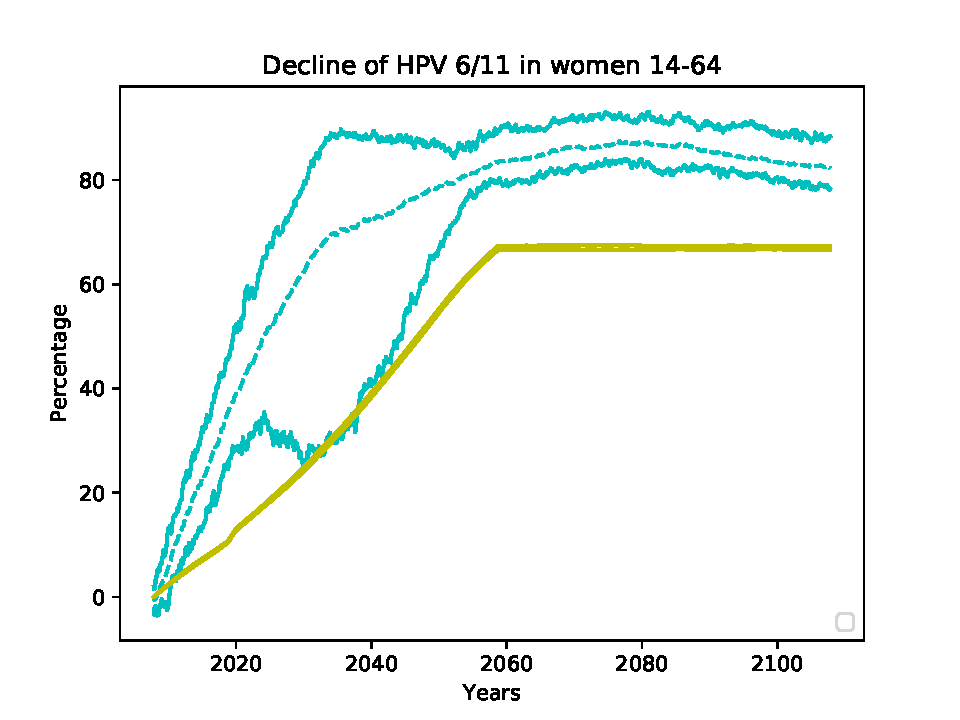
\includegraphics[width=0.5\linewidth]{IMGs/4.-Decline_verrugas/verr_muj.pdf}	& 
		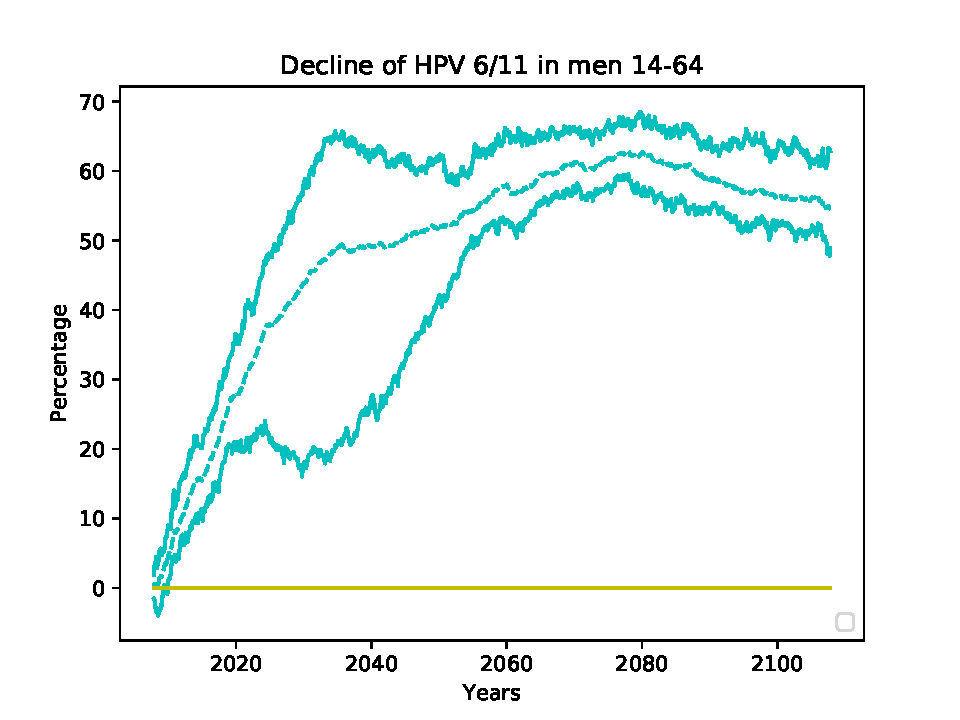
\includegraphics[width=0.5\linewidth]{IMGs/4.-Decline_verrugas/verr_hom.pdf}  \\ 
		(a)	& (b) \\ 
		\multicolumn{2}{c}{ 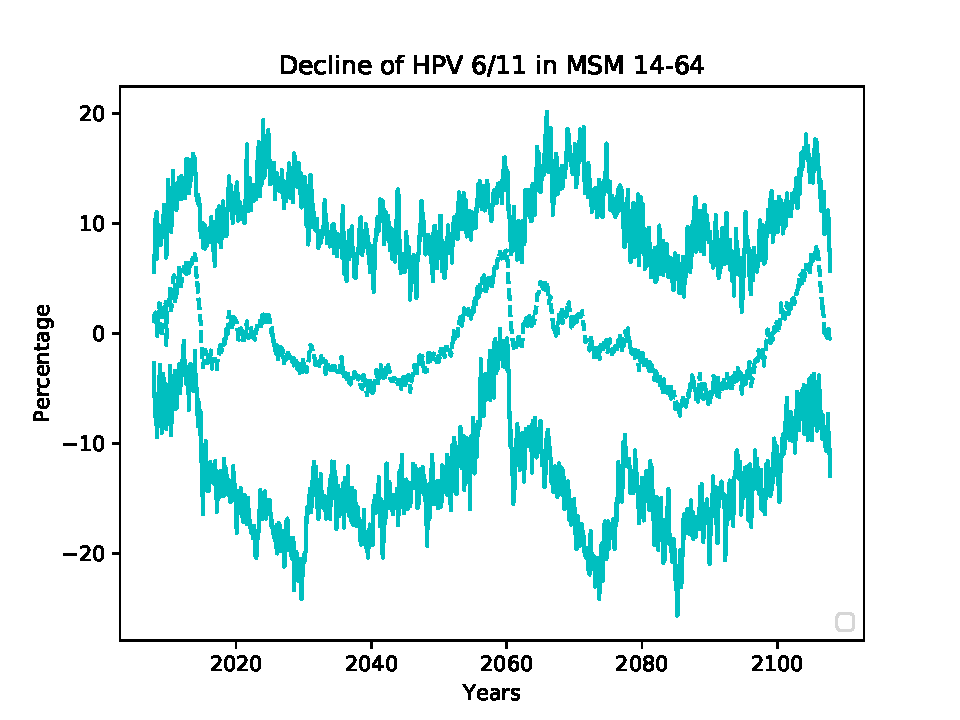
\includegraphics[width=0.5\linewidth]{IMGs/4.-Decline_verrugas/verr_MSM.pdf} } \\ 
		\multicolumn{2}{c}{(c)} \\ 
	\end{tabular} 
	\caption{Decline of HPV LR 6/11 infections, and consequently, of genital warts (GW) in 14-64 years old women (a), men (b) and MSM (c) over the time, from Oct 2007 when the vaccination campaign started in Spain. In the women decline, we include the percentage of vaccinated women. It helps to visualize the herd immunity effect when the decline line is over the vaccination line. In case of men, the lines over the yellow abscissa line means effect of the herd immunity. However, for the MSM, as in the Australian case, there is not herd immunity effect.}
	\label{fig:verrESP}
\end{figure}

The differences between the best and the worst cases is due to the LSP network structure. We do not know exactly how these networks are and the uncertainty that involves the building of these networks may lead to extreme scenarios. This happens in general and in MSM in particular. Thus, we should say that, in our built networks of $100,000$ nodes, less than $2,000$ are labeled MSM. This figure is very low to state predictions for MSM population with a reliable uncertainty and it may explain why the Figure \ref{fig:verrESP} for MSM has so extreme $95\%$ confidence interval.

In the Table \ref{tabla:verrESP}, we can see when given percentages of decline will be reached for women and men. Note that it is not necessary a long time to achieve high percentages of decline for women and men.

\begin{table}[!h]
\centering
\begin{tabular}{c|ll}
	Decline & Women & Men  \\ 
	\hline 
$ 30 \%$ & year  2017 , CI95\% $[ 2015 , 2035 ]$ & year  2021 , CI95\% $[ 2018 , 2044 ]$  \\
$ 40 \%$ & year  2021 , CI95\% $[ 2017 , 2039 ]$ & year  2027 , CI95\% $[ 2023 , 2049 ]$  \\	
$ 50 \%$ & year  2024 , CI95\% $[ 2020 , 2045 ]$ & year  2044 , CI95\% $[ 2027 , 2103 ]$  \\
$ 60 \%$ & year  2029 , CI95\% $[ 2023 , 2047 ]$ & year  2068 , CI95\% $[ 2055 , - ]$  \\
$ 70 \%$ & year  2035 , CI95\% $[ 2027 , 2052 ]$ & year  $-$ , CI95\% $[ - , - ]$  \\
$ 80 \%$ & year  2053 , CI95\% $[ 2030 , 2101 ]$ & year  $-$ , CI95\% $[ - , - ]$  \\
\end{tabular} 
\caption{In this table we show when given percentages of decline of HPV LR 6/11 will be reached over the time with a $95\%$ confidence interval. The symbol "$-$" means that this percentage is not reached in the simulation period. Note that, in average, high percentages of decline for women and men are achieved very soon.}
\label{tabla:verrESP}
\end{table}

